%Appunti del Corso Computabilità
\documentclass[a4paper]{book}
\usepackage[T1]{fontenc}%per rappresentare i font italiani, come le lettere accentate, con la giusta spaziatura
\usepackage[utf8]{inputenc}%per poter inserire nel testo .tex i caratteri unicode8
\usepackage[italian]{babel}%per poter effettuare la giusta sillabazione della lingua italiana
\usepackage{classicthesis}%necessario per usare lo stile arsclassica
\usepackage{arsclassica}%per poter usare lo stile arsclassica usato nell'Arte di imparare il Latex
\usepackage{amsmath}%per poter rappresentare ed utilizzare al meglio gli ambienti e le formule matematiche
\usepackage{amssymb}%per rappresentare alcuni simboli particolari matematici
\usepackage{amsthm}%per definire e poter effettuare le dimostrazioni matematiche
\usepackage{amsfonts}%per poter avere i font matematici
\usepackage{amstext}%per avere una gestione del testo nell'ambiente matematico
\usepackage{booktabs}%per la corretta gestione delle tabelle
\usepackage{graphics}%per effettuare i grafici
\usepackage{rotating}%per effettuare le rotazioni delle immagini e grafici
\usepackage{microtype}%per effettuare un aggiustamento della spaziatura tra caratteri e del font
\usepackage{tikz}%Pacchetto per fare i disegni in particolare con la libreria automata farò gli automi
\usetikzlibrary{automata,positioning}%libreria per disegnare automi a stati finiti

\theoremstyle{definition}%per avere lo stile tondo quando uso un ambiente definito da newtheorem
\newtheorem*{defi}{Def}%Definizione per avere la gestione delle definizioni
\newtheorem{prop}{Prop}[chapter]
\newtheorem{lem}{Lemma:}
\newtheorem{thm}{Thm:}[chapter]
\newtheorem{corol}{Corol}[chapter]
\newtheorem*{esempio}{Esempio}
\newcommand{\numberset}{\mathbb}
\newcommand{\N}{\numberset{N}}

\begin{document}

\title{Appunti del corso Linguaggi e Computabilità}
\author{Marco Natali}
\date{}
\maketitle

Il corso di Linguaggi e Computabilità riguarda l'informatica teorica e si occupa di definire la calcolabilità di un problema,
di definire le grammatiche e i linguaggi formali con l'ausilio di anche di automi e macchine di Turing.

Incominciamo con la definizione dei componenti basilari attraverso cui svilupperemo poi i concetti del corso
\begin{defi}
  Si definisce come \emph{alfabeto}, indicato con $\Sigma$, una sequenza di simboli, attraverso cui possiamo stabilire un alfabeto.\newline
  Si definisce invece come stringa, una sequenza finita di simboli appartenenti ad un alfabeto $\Sigma$ ed esisterà sempre la stringa $\epsilon$,
  indicante la stringa vuota.
\end{defi}
\begin{esempio}
  \[
  \begin{aligned}
    \Sigma = \{0, 1\}\ \text{e} \Sigma = \{a, b, c\} \\
    w = 10110 \, \, \, z = abccabbcc \\
  \end{aligned}
  \]
\end{esempio}
\begin{defi}
È possibile fornire una definizione induttiva di stringa, partendo dalla stringa $\epsilon$:
    \begin{description}
      \item [caso base]: $\epsilon$ è una stringa vuota
      \item [caso passo]: se $w$ è una stringa, allora anche $a \circ w $ è una stringa
    \end{description}
\end{defi}
Dopo aver fornito le definizioni per le stringhe, definiamo le seguenti operazioni definite su le stringhe:
\begin{itemize}
   \item insieme di stringhe: definiamo come $\Sigma ^ k$ l'insieme di stringhe su $\Sigma$ con $k$ caratteri come segue:
          \[
          \begin{aligned}
          \Sigma ^ 0 & = \{ \epsilon\} \\
          \Sigma ^ 1 & \neq \Sigma \text{ma sono l'insieme delle stringhe di un carattere} \\
          \Sigma ^ 2 & = \text{insieme di stringhe di due caratteri} \\
          \dots \dots \\
          \Sigma ^ k & = \text{insieme di stringhe di k caratteri} \\
          \end{aligned}
          \]
        Le due più importanti insiemi di stringhe, usate per rappresentare l'insieme di stringhe di qualsiasi lunghezza, sono:
        \[
        \begin{aligned}
          \Sigma ^ * & = \cup _{i = 0} \Sigma ^ i \\
          \Sigma ^ + & = \Sigma ^ * - \{\epsilon\} \\
        \end{aligned}
        \]

  \item $|w|: \Sigma ^ * \to \N$: rappresenta la lunghezza di una stringa, ossiail numero di caratteri presenti in una stringa,
        e la definizione di lunghezza avviene induttivamente come segue:
        \begin{description}
        \item [base]: la lunghezza di $|\epsilon| = 0$
        \item [passo]: se $|w| = n$ con $n \in \N$ e sia $a \in \Sigma$ allora $|a \circ w| = 1 + |w| = n + 1$.
        \end{description}
        \begin{esempio}
          $w = abcdec  \quad |w| = 6$
        \end{esempio}

  \item $\circ: \sum ^ * \times \sum ^ * \to \sum ^ *$: rappresenta la concatenazione, ossial'aggiunta dei caratteri della seconda stringa
        al termine della prima stringa ma vediamo ora una definizione più formale:
        \begin{defi}
          Date due stringhe $x = a_1 a_2 \dots a_n$ e $y = b_1 b_2 \dots b_n$ si definisce $x \circ y = a_1 a_2 \dots a_n b_1 b_2 \dots b_n$
          con $|x \circ y| = |x| + |y| = n + m$.
        \end{defi}
        La concatenazione possiede le seguenti proprietà:
        \begin{itemize}
        \item è associativa: $\forall x,y,z \in \sum^* x \circ (y \circ z) = (x \circ y) \circ z$.
        \item non è commutativa infatti presi due stringhe $x,y$ diverse risulta $x \circ y \neq y \circ x$.
        \item possiede l'elemento neutro $\epsilon$ per cui $x \circ \epsilon = x = \epsilon \circ x$.
        \end{itemize}
        \begin{esempio}
          \begin{equation*}
          \begin{split}
            w = 1011100 \quad z = 1011110  \\
          w \circ z & = 10111001011110 \\
          z \circ w  &= 10111101011100 \\
          \end{split}
          \end{equation*}
        \end{esempio}
  \end{itemize}
Attraverso le seguenti operazioni si può stabilire che $(\Sigma ^ *,\circ,\epsilon)$ è un monoide libero su $\Sigma$.

Dopo aver considerato e definito l'alfabeto e le stringhe, bisogna definire i linguaggi, concetto su cui si basa tutto il nostro
corso e l'informatica teorica:
\begin{defi}
    Definiamo come \emph{Linguaggio} un'insieme di stringhe scelte su $\Sigma ^ *$ scelte per far parte del linguaggio
    ossia $L \subseteq \Sigma ^ *$.
    Le componenti di un linguaggio sono:
    \begin{description}
    \item [alfabeto] : insieme di simboli su cui definiamo poi il lessico e la sintassi
    \item [lessico]: definisce il vocabolario del linguaggio e viene definito tramite una grammatica di tipo 3
    \item [sintassi]: definisce come le varie frasi del linguaggio devono essere disposte nel linguaggio e ciò
      viene definito da una grammatica di tipo 2.
    \item [semantica]: il significato attribuito alle frasi del linguaggio però nei linguaggi formali deriva dalla sintassi
      anche se in questo corso la semantica non verrà affrontata.
    \end{description}
\end{defi}
I linguaggi possono essere riconosciuti attraverso degli automi oppure generati medianti delle grammatiche.\newline
Un'altra cosa importante è che si hanno sottoinsiemi particolari di linguaggi, come l'insieme vuoto, che resta comunqe un linguaggio,
il \textbf{linguaggio vuoto} e $\emptyset \in \Sigma^k,\,|\emptyset|=0$ che è diverso dal linguaggio che contiene la stringa vuota $|\epsilon|=1$,
inoltre $\Sigma^*\subseteq \Sigma^*$ che ha lunghezza infinita.\newline
Vediamo qualche esempio di linguaggio:
\begin{itemize}
\item il linguaggio di tutte le stringhe che consistono in $n$ 0 seguiti da $n$ 1:
  \[ \{\epsilon,01,0011,000111,...\} \]
\item l'insieme delle stringhe con un uguale numero di 0 e di 1:
  \[ \{\epsilon,01,10.0011,0101.1001,..\} \]
\item l'insieme dei numeri binari il cui valore è un numero primo:
  \[ \{\epsilon,10 , 11, 101, 111,1011,...\} \]
\item $\Sigma^*$ è un linguaggio per ogni alfabeto $\Sigma$
\item $\emptyset$, il linguaggio vuoto, e $\{\epsilon\}$ sono un linguaggio rispetto a qualunque alfabeto
\end{itemize}
La prima modalità per definire un linguaggio è attraverso la definizione di una grammatica, per stabilire tutte e sole
le stringhe del linguaggio.
In questo paragrafo forniremo soltanto una definizione informale e definiamo le diverse tipologie di gerarchie, senza
effettuarne una trattazione formale, cosa che avverrà nel prossimo capitolo.
\begin{defi}
    Si definisce come \emph{Grammatica} un'insieme di regole che delineano le stringhe ammissibili del linguaggio e
    possono essere di due tipologie:
    \begin{itemize}
      \item grammatica generativa : insieme di regole che permettono di generare tutte le stringhe di un lunguaggio partendo dalle stringhe base
      \item grammatica analitica : analizza le stringhe passate in input e stabilisce l'appartenenza o meno al linguaggio
    \end{itemize}
\end{defi}
  Nel 1956 il linguista Choumsky introdusse e definì la gerarchia delle grammatiche e linguaggi, che ha avuto una notevole importanza
  nell'informatica teorica anche se il suo intento era quello di catalogare le varie tipologie di linguaggi naturali:
\begin{description}
  \item [grammatiche di tipo 0]: non si hanno restrizioni sulle regole di produzione, $\alpha\to\beta$ e sono linguaggi ricorsivamente numerabili,
    rappresentati dalle \emph{macchine di Turing}, deterministiche o non deterministiche (la macchina di Turing è un automa).

  \item [grammatiche di tipo 1]:  il lato destro della produzione ha lunghezza almeno uguale a quello sinistro e si chiamano anche
        grammatiche dipendenti dal contesto e come automa hanno \emph{la macchina di Turing che lavora in spazio lineare}:
        \[ \alpha_1A\alpha_2\to \alpha_1B\alpha_2 \]
        con $\alpha_1$ e $\alpha_2$ detti \emph{contesto} e $\alpha_1,\,\alpha_2,\, \beta\in (V\cup T)^*$

  \item [grammatiche di tipo 2]: sono quelle libere dal contesto, context free ed usano come riconoscitore gli automi a pila.
        Come regola ha $A\to\beta$ con $A\in V$ e $\beta\in V\cup T)^*$.

  \item [grammatiche di tipo 3]: sono le grammatiche \emph{regolari}, i cui linguaggi vengono riconosciuti dagli automi a stati finiti.\newline
        Come regole ha $A\to\alpha B$ (o $A\to B\alpha$) e $A\to\alpha$  con $A,B\in V$ e $\alpha\in T$.
\end{description}
Durante questo corso effettueremo una trattazione delle grammatiche di tipo 3 e 2, anche se analizzeremo solo un esempio di grammatica di tipo 1;
iniziamo nel prossimo capitolo a considerare le grammatiche di tipo 2, chiamate grammatiche context-free.

\chapter{Grammatiche di tipo 2}
Iniziamo ora a considerare le grammatiche di tipo 2 partendo da un esempio e poi fornendo una definizione formale.
\begin{esempio}
  Dato il linguaggio delle stringhe palindrome $L _{pal} = \{w \in \Sigma ^ * : w = w ^ R\}$ dove $w^R$ rappresenta la stringa
  reversa per cui ad esempio $'OTTO' \in L_{pal}$ mentre $'PAPA'$ non appartiene al linguaggio.

  Definiamo in maniera più formale e meno ambigua i componenti di $L_{pal}$:
  \begin{description}
  \item [caso base]: $\epsilon, 0, 1 \in L_{pal}$
  \item [caso induttivo]: se $w \in L_{pal}$ allora $0w0$ e $1w1$ appartengono a $L_{pal}$ e nient'altro appartiene al linguaggio.
  \end{description}
  Le regole di derivazione per $L_{pal}$ sono le seguenti, e derivano dalla definizione dei componenti:
  \begin{itemize}
  \item $P \to \epsilon$
  \item $P \to 0$
  \item $P \to 1$
  \item $P \to 0P0$
  \item $P \to 1P1$
  \end{itemize}
  Una versione più concisa delle regole di derivazione è la seguente:
  \[ P_g\{P \to \epsilon | 0 | 1 | 0P0 | 1P1\} \]
  Dopo aver dato le regole di derivazione dobbiamo capire se le seguente regole definiscono tutte e sole le stringhe del linguaggio per
  cui ci chiediamo per esempio se $010 \in L_{pal}$ e $10001 \in L_{pal}$?
  \begin{align}
    P \Rightarrow 0P0 \Rightarrow 010  \quad \text{la stringa appartiene correttamente al linguaggio}\\
    P \Rightarrow 1P1 \Rightarrow 10P01 \Rightarrow 10001 \quad \text{la stringa appartiene correttamente al linguaggio}\\
  \end{align}
  Attraverso l'applicazione di una serie di regole di derivazione otteniamo una stringa $w \in \Sigma ^*$ se e solo $w \in L$
  della grammatica definita.
\end{esempio}

%Definizione di Grammatica
\begin{defi}
  Si definisce una grammatica context free come $G = (V, T, P_g, S)$, i cui componenti sono:
  \begin{itemize}
  \item $V$ rappresenta l'insieme delle variabili usate per rappresentare un linguaggio
  \item $T$ rappresenta l'insieme dei simboli terminali, ossia l'insieme dei simboli attraverso cui sono definite le stringhe
    del linguaggio per questo di solito coincide con l'alfabeto del linguaggio.

  \item $S$ rappresenta la variabile di inizio della grammatica, ossia la variabile attraverso cui si definisce la grammatica
    per cui le altre variabili sono classi ausiliari di stringhe che aiutano a definire le stringhe del linguaggio.

  \item $P_g$ indica l'insieme di regole, che rappresentano la definizione ricorsiva del linguaggio, della seguente forma:
    \begin{equation*}
        P_g = \{ X \to \beta | \beta \in (V \cup  T)^* \ \text{e} \ X \in V\}
    \end{equation*}
    la variabile $X$ rappresenta la testa della produzione mentre $\beta$ è il corpo
  \end{itemize}
  Non si possono applicare delle regole in parallelo, ma soltanto una alla volta.
\end{defi}

  Nell'esempio del linguaggio palidromo la grammatica che lo genera è
  \begin{equation*}
    G = (\{P\},\{0, 1\}, \{P \to \epsilon,P \to 0,P \to 1,P \to 0P0,P \to 1P1\}, S\}
  \end{equation*}

  %Concetto di derivazione
  Dopo aver definito in maniera formale di grammatica introduciamo il concetto di derivazione, per stabilire se una stringa appartiene
  o meno al linguaggio.
  \begin{defi}
    Sia $G = (V, T,P_g,S)$ una grammatica context-free, sia $\alpha A \beta$ una stringa di terminali e variabili con $A \in V$ e
    sia infine $A \to \gamma$ una regola di derivazione allora $\alpha A \beta \Rightarrow _g \alpha \gamma \beta$.\newline
    Si indica $\Rightarrow _g ^*$, il simbolo di applicazione di zero,uno o più step di derivazione, definito nel seguente modo:
    \begin{description}
    \item [caso base]: per ogni stringa $\alpha$ di terminali e variabili, si ha $\alpha \Rightarrow _g ^* \alpha$
    \item [caso passo]: se $\alpha \Rightarrow _g ^* \beta$ e $\beta \Rightarrow _ g \gamma$ allora $\alpha \Rightarrow _g ^* \gamma$
    \end{description}
    Si può anche dire che $\alpha\to_G *\, \beta$ se e solo se esiste una sequenza di stringhe $\gamma_1,...,\gamma_n$ con $n\geq 1$
    tale che $\alpha=\gamma_1$, $\beta=\gamma_n$ e $\forall i,\, 1<i<n-1$ si ha che $\gamma_1\to \gamma_{i+1}$ per cui
    la derivazione in 0 o più passi è la chiusura transitiva della derivazione.
  \end{defi}
  Le stringhe che otteniamo sono delle forme sentenziali, ossia stringhe appartenenti a $(V \cup T)^*$ e un particolare
  sottoinsieme, in cui le stringhe sono composte soltanto da terminali, definisce le stringhe del linguaggio.

  Sempre considerando l'esempio del linguaggio delle stringhe palindrome la derivazione di $10011001$ è la seguente:
  \begin{equation*}
    P \Rightarrow 1P1 \Rightarrow 10P01 \Rightarrow 100P001 \Rightarrow 1001P1001 \Rightarrow 10011001
  \end{equation*}

  Al fine di ridurre il numero di scelte nella derivazione di una stringa introduciamo ora:
  \begin{description}
  \item [left derivation]: sostituiamo la variabile più a sinistra nell'applicazione di una regola di derivazione
                           e ciò viene rappresentato con il simbolo $\Rightarrow _{lm}$.

  \item [right derivation]: sostituiamo la variabile più a destra nell'applicazione di una regola di derivazione
                            ed essoviene rappresentato con il simbolo $\Rightarrow _{rm}$.
  \end{description}

  \begin{defi}
    Data una grammatica context-free $G = (V, T, P_g, S)$ si definisce un linguaggio context-free $L$ come:
    \begin{equation*}
      L_g = \{ w \in T^* | S \Rightarrow _g ^* w \}
    \end{equation*}
  \end{defi}

  Nei linguaggi context-free si può soltanto effettuare la concatenazione e l'annidamento dei sottolinguaggi come vediamo
  nei seguenti esempi:

  %Esempio di linguaggio Context-free
  \begin{esempio}
  Mostriamo ora un esempio di linguaggio definito come la concatenazione di due linguaggi
  \begin{equation*}
     L_g = \{ w \in \{0,1\}^* | w = 0^m 1^{m+1}01^n001^n \ n\geq 0\}
  \end{equation*}
  Si può vedere che ci 3 blocchi che concatenati generano il linguaggio $L_g$ per cui le regole di derivazione sono
  \[ P_g = \{S \to X0Y, X \to 1 | 0X1, Y \to 1001 | 1Y1\} \]
  \end{esempio}
  \begin{esempio}
    Mostriamo ora un esempio di linguaggio definito come l'annidamento di linguaggi:
    \begin{equation*}
      L = \{ w = \{a,b,c,d\}^* | w = a^nb^mc^md^n \, m > 0, n \geq 0\}
    \end{equation*}
    Le regole di produzione del seguente linguaggio sono $P_g = \{S \to aSd | Y, Y \to bYc | bc\}$
    e come si nota il linguaggio viene definito come una sequenza di a e d intrammezzate da un blocco Y, formato da b e c,
    e ciò è l'annidamento tra diversi blocchi di una stringa che formano le stringhe del linguaggio.
  \end{esempio}

  %Inferenza Ricorsiva
  Un'altra modalità per stabilire l'appartenza di una stringa di un linguaggio è l'\emph{inferenza ricorsiva}, in cui, a differenza delle altre
  modalità, applica le regole dal corpo alla testa, ossia concateniamo ogni terminale che appare nel corpo e inferiamo che la stringa trovata
  è nel linguaggio delle variabili, presenti in testa alle regole.

  Viene poco utilizzato in quanto è più naturale e chiaro pensare secondo la derivazione per cui ne vediamo soltanto un esempio
  e lo usiamo in un importante teorema sull'equivalenza delle modalità di derivazione, che verrà presentato prossimamente.
  \begin{esempio}
    Sia $G=(V,T,O,E)$, con $V=\{E,I\}$ e $T=\{a,b,0,1,(,),+,*\}$
    quindi ho le seguenti regole, è di tipo 3:
    \begin{enumerate}
    \item $E\to I | E+E | E*E | (E)$
    \item $I\to a | b | Ia | Ib | I0 | I1$
    \end{enumerate}
    Voglio ottenere $a*(a+b00)$ e sostituisco sempre a destra (right most derivation):
    \[E\to E*E\to E*(E)\to E*(E+E)\to E*(E+I)\to E+(E+I0)\]
    \[\to R+(I+b00)\to E*(a+b00)\to I*(a+b00)\to a*(a+b00)\]
    usiamo ora \textit{l'inferenza ricorsiva}:
    \begin{table}
      \centering
    \caption{Inferenza ricorsiva di $a*(a+b00)$}
      \begin{tabular}{|c|c|c|c|c|}
        \toprule passo & stringa ricorsiva & var & prod & passo stringa impiegata\\
        \midrule 1 & a & I & 5 & $\backslash$ \\
        \hline
        2 & b & I & 6 & $\backslash$ \\
        \hline
        3 & b0 & I & 9 & 2\\
        \hline
        4 & b00 & I & 9 & 3\\
        \hline
        5 & a & E & 1 & 1 \\
        \hline
        6 & b00 & E & 1 & 4\\
        \hline
        7 & a+b00 & E & 2 & 5,6\\
        \hline
        8 & (a+b00) & E & 4 & 7\\
        \hline
        9 &a*(a+b00) & E & 3 & 5, 8\\
        \hline
      \end{tabular}
    \end{table}
  \end{esempio}

  %Alberi Sintattici
\section{Alberi di Derivazione}
Introduciamo ora un'importante forma grafica per vedere le regole di derivazioni applicate per formare una stringa
\begin{defi}
    Data una grammatica context-free $G$, un albero di derivazione per $G$ è un albero composto come:
    \begin{itemize}
       \item ogni nodo interno è etichettato con una variabile $X \in V$, con la radice etichettata con $S$.
       \item ogni foglia è etichettata con una variabile, un simbolo terminale o $\epsilon$; se una foglia viene etichettata
             con $\epsilon$ allora dev essere l'unico figlio del padre.
       \item se un nodo è etichettato con $A$ e i suoi figli sono etichettati come $x_1, x_2, \dots, x_k$, allora $A \to x_1x_2 \dots x_k$
             è una regola di produzione della grammatica.
    \end{itemize}
  \end{defi}
Eseguendo la concatenazione delle stringhe foglia otteniamo una stringa $w$ appartenente alla grammatica di cui abbiamo svolto l'albero sintattico
  %Esempio di Albero Sintattico
  \begin{esempio}
    Prendendo il linguaggio $L$ definito come segue:$L = \{w \in \{a,b,c,d\}^* | w = a^ncb^mcd^{n+m} n \geq 0,m > 0\}$
    stabiliamo una grammatica context-free e fare l'albero sintattico di $aacbbbcddddd \in L$:
    le regole di produzione di $L$ sono $P_g = \{S \Rightarrow aSd | cY, Y \Rightarrow bcd | bYd\}$ per cui la grammatica è:
    \begin{equation*}
      G = (\{S,Y\},\{a,b,c,d\},P_g,S)
    \end{equation*}
    L'albero sintattico di $aacbbbcddddd$ è il seguente:

  \end{esempio}

  \section{Equivalenza tra le derivazioni}
  In questo paragrafo consideriamo un importante teorema sulle equivalenze tra le varie modalità di derivazione, definito come segue:
  \begin{thm}
    Data una grammatica context-free $G = (V, T,P_g,S)$ abbiamo che le seguenti modalità di derivazione sono equivalenti:
    \begin{enumerate}
    \item la procedura di inferenza ricorsiva che determina che una stringa di terminali $w$ appartiene ad un linguaggio di variabili $A$
    \item $A \Rightarrow ^ * w$
    \item $A \Rightarrow _{lm} ^ * w$
    \item $A \Rightarrow _{rm} ^ * w$
    \item esiste un albero sintattico con radice $A$ e come prodotto di foglie la stringa $w$.
    \end{enumerate}
  \end{thm}
  \begin{esempio}
Usiamo l'esempio delle stringhe palindrome:
$$P\to 0P0|\,1P1|\epsilon$$
sia il seguente albero sintatico:
\end{esempio}

\begin{esempio}
Si ha:
$$E\to I|\, E+E|\, E*E|\, (E)$$
$$I\to a|\,b|\,Ia|\,Ib|\,I0|\,I1$$
un albero sintattico per $a*(a+b00)$ può essere:
\end{esempio}


queste 5 proposizioni si implicano l'uni l'altra:
\begin{center}
\begin{tikzpicture}
    \node (top) at (0,0) {5};
 	\node (a) at(-1,-0.5) {3};
 	\node (b) at(0,-1) {4};
 	\node (c) at(-2.0,-1.85) {2};
 	\node (d) at(1.5,-2) {1};
    \draw [->] (top) -- (a);
    \draw [->] (top) -- (b);
    \draw [->] (a) -- (c);
    \draw [->] (b) -- (c);
    \draw [->] (c) -- (d);
    \draw [->] (d) -- (top);
\end{tikzpicture}
\end{center}
Le prime due sono banali dato che una derivazione sinistra/destra sono anche delle derivazioni quindi risulta verificato.
Vediamo le altre dimostrazioni di implicazioni:
\begin{proof}[da 1 a 5]
si procede per induzione:
\begin{itemize}
\item \textbf{caso base:} ho un livello solo (una sola riga), $\exists A\to w$:
$$\overset{A}{\overset{\triangle}w}$$
\item \textbf{caso passo:} suppongo vero per un numero di righe $\leq n$, lo dimsotro per $n+1$ righe:
$$A\to X_1,X_2,...,X_k$$
$$w=w_1,w_2,...,w_k$$
ovvero, in meno di $n+1$ livelli:
\end{itemize}
\end{proof}
\begin{proof}[da 5 a 3]
procedo per induzione:
\begin{itemize}
\item \textbf{caso base (n=1): }$\exists A\to w\mbox{ quindi } A\to_{lm}w$, come prima si ha un solo livello:
$$\overset{A}{\overset{\triangle}w}$$
\item \textbf{caso passo: }suppongo che la proprierà valga per ogni albero di profondità minore uguale a $n$, dimostro che valga per gli alberi profondi $n+1$:
$$A\to X_1,X_2,...,X_k$$
$$w=w_1,w_2,...,w_k$$
ovvero, in meno di $n+1$ livelli:
\begin{center}

%\psframebox[linestyle=none,framesep=10pt]{%
%pstree{\LFTw{t}{\fontspec{Noto Sans}[Script=Latin]A}}{\pstree{\Tp[edge=none]}{%
%  \LFTw{t}{\fontspec{Noto Sans}[Script=Latin]$\overset{X_1}{\overset{\triangle}w_1}$}
%  \LFTw{t}{\fontspec{Noto Sans}[Script=Latin]$\overset{X_2}{\overset{\triangle}w_2}$}
%  \LFTw{t}{\fontspec{Noto Sans}[Script=Latin]$\vdots$}
%  \LFTw{t}{\fontspec{Noto Sans}[Script=Latin]$\overset{X_k}{\overset{\triangle}w_k}$}}}}
\end{center}
$$A\to_{lm} X_1,X_2,...,X_k$$
$$x_1\to^*_{lm}w_1 \mbox{ per ipotesi induttiva si ha un albero al più di n livelli}$$
quindi:
$$A\to_{lm}X_1,...,X_k\to^*_{lm}w_1,X_2,...,X_k\to^*_{lm}...\to^*_{lm}w_1,...,w_k=w$$
\end{itemize}
\begin{esempio}
$$E\to I\to Ib\to ab$$
$$\alpha E\beta\to\alpha I\beta\to \alpha Ib\beta\to \alpha ab\beta,\,\,\,\alpha,\beta\in(V\cup T)^*$$
\end{esempio}
\end{proof}
\begin{esempio}
Mostro l'esistenza di una derivazione sinistra dell'albero sintattico di $a*(a+b00)$:
$$E\to^*_{lm}E*E\to^*_{lm}I*E\to^*_{lm}a*E\to^*_{lm}a*(E)\to^*_{lm}a*(E+E)\to^*_{lm}$$
$$a*(I+E)\to^*_{lm}a*(a+E)\to^*_{lm}a*(a+I)\to^*_{lm}a+(a+I0)\to^*_{lm}a*(a+I00)\to^*_{lm}a*(a+b00)$$
\end{esempio}

\section{Grammatiche e Linguaggi Ambigui}
Fino ad ora abbiamo considerato delle grammatiche uniche, ossia in grado di generare in maniera univoca un linguaggio ma non è sempre così,
infatti in questo paragrafo consideramo il problema dell'ambiguità nelle grammatiche e nelle grammatiche.

Diamo ora una definizione formale di grammatica ambigua:
  \begin{defi}
    Si dice che una grammatica è ambigua se e solo se esiste una stringa $w \in L$ tale per cui $w$ ammette due derivazioni $lm$ e/o $rm$
    diverse oppure ammette due alberi sintattici definiti sulla stessa grammatica $G$
  \end{defi}
  L'obiettivo è quello di avere grammatiche non ambigue perchè esse permettono di definire in maniera univoca, per cui automamilizzabile
  con una procedura, l'insieme delle stringhe del linguaggio e fortunatamente nella maggior parte dei casi, quando il linguaggio non è ambiguo,
  data una grammatica ambigua è possibile definire una grammatica non ambigua $G'$ tale che $L(G) = L(G')$.
\begin{esempio}
vediamo un esempio:

La grammatica data delle espressioni algebriche ha due cause di ambiguità:
\begin{enumerate}
  \item la precedenza degli operatori non viene rispettata in quanto andrebbe raggruppato prima il silmbolo di $*$ rispetto a $+$
  \item una sequenza di uguali operatori può essere reggruppata sia da sinistra che da destra e si stabilisce per convenzione
    che si raggruppa da sinistra a destra.
\end{enumerate}
  Considerate queste cause di ambiguità, per eliminarla si introducono altre variabili definite come:
  \begin{enumerate}
  \item un fattore è un espressione che non può essere spezzata da nessun operatore, sia il $*$ che il $+$, per cui gli unici fattori
    nel nostro linguaggio delle espressioni sono gli identificatori e ogni espressioni dentro le parentesi.
  \item un termine è un espressione che non può spezzata dall'operatore $+$.
  \item un espressione può riferirsi a qualsiasi possibile espressione, incluse quelle che possono essere spezzate da un adiacente $*$ o $+$
  \end{enumerate}
  La grammatica non ambigua del linguaggio delle espressioni è la seguente:
  \begin{equation*}
    P_{exp} = \{E \to T | E + T, T \to F | T * F,F \to I | (E), I \to a | b | aI| bI | 0I | 1I\}
  \end{equation*}
\end{esempio}
Possono esserci più derivazioni di una stringa ma l'importante è che non ci siano alberi sintattici diversi e capire se una CFG è ambigua
è un problema indecidibile, per cui molto complesso ed oneroso.
\begin{esempio}
vediamo un esempio:
\[ S\to \epsilon|\,SS|\, iS|\, iSeS \]
con S=statement, i=if e e=else.
Considero due derivazioni:
\begin{enumerate}
\item $S\to iSeS\to iiSeS\to iie$:
  Fare albero sintattico!!!!
\end{enumerate}
Si ha quindi una grammatica ambigua
\end{esempio}
Per risolvere codesto problema nei linguaggi di programmazione i compilatori assumono la consecutine di associare l'else all'ultimo if

 \begin{defi}
    Un linguaggio $L \subseteq \sum^*$ è detto \emph{ambiguo} se per ogni grammatica $G$, tale per cui $L = L_G$, risulta che $G$ è ambigua.
  \end{defi}
\begin{esempio}
Sia $L=\{a^nb^nc^md^m|\, n,m\geq 1\}\cup \{a^nbmnc^md^n|\, n,m\geq 1\}$\\
si ha quindi un CFL formato dall'unione di due CFL. $L$ è inerentemente ambiguo e generato dalla seguente grammatica:
\begin{itemize}
\item $S\to AB|\,C$
\item $A\to aAb|\,ab$
\item $B\to cBd|\, cd$
\item $C\to aCd|\, aDd$
\item $D\to bDc|\, bc$
\end{itemize}
si possono avere due derivazioni:
\begin{enumerate}
\item $S\to_{lm}AB\to_{lm} aAbB\to_{lm} aabbB\to_{lm}aabbcBd\to_{lm}aabbccdd$
\item $S\to_{lm} C\to_{lm} aCd\to_{lm}aaBdd\to_{lm}aabBcdd\to_{lm}aabbccdd$
\end{enumerate}
a generare problemi sono le stringhe con n=m perché possono essere prodotte in due modi diversi da entrambi i sottolinguaggi. Dato che l'intersezione tra i due sottolinguaggi non è vuota si ha che $L$ è ambiguo
\end{esempio}

\chapter{Linguaggi e grammatiche dipendenti dal contesto}
vediamo un esempio di grammatica dipendente dal contesto:
\[L=\{a^nb^nc^n|\, n\geq 1\} \text{la cui grammatiche che lo genera è la seguente:} \]
\[ G=\{V,T,P,S\}=\{(S,B,C,X)\}=\{(a,b,c),P,S\}\].\newline
Ecco le regole di produzione, e le grammatiche di tipo 1 posso scambiare variabili a differenza delle context free:
\begin{enumerate}
\item $S\to aSBC$
\item $S\to aBC$
\item $CB\to XB$
\item $XB\to XC$
\item $XC\to BC$
\item $aB\to ab$
\item $bB\to bb$
\item $bC\to bc$
\item $cC\to cc$
\end{enumerate}
Vediamo un esempio di derivazione:
per $n=1$ ho $abc$ ovvero $S \to aBC \to abC \to abc$.\newline
con $n=2$ ho $aabbcc$:
\[ S\to aSBC\to aaBCBC\to aaBXBC\to aaBXCC\to aaBBCC\to aabBCC\to aabbCC\to aabbcC\to aabbcc \]
Vedere dimostrazione pag 14 di Lorenzo Soligo
%vedere dimostrazione pag 14 soligo
Vediamo un esempio di grammatica dipendente dal contesto:
\[ L=\{a^nb^mc^nd^m|\, n,m\geq 1\} \]
Si ha:
\[ G=(\{S,X,C,D,Z\},\{a,b,c,d\},P,S) \]
con le seguenti regole di produzione:
\begin{itemize}
\item $S\to aSc|\, aXc$
\item $X\to bXD|\, bD$
\item $DC\to CD$
\item $DC\to DZ$
\item $DZ\to CZ$
\item $XZ\to CD$
\item $bC\to bc$
\item $cC\to cc$
\item $cD\to cd$
\item $dD\to dd$
\end{itemize}
Provo a derivare $aabbbccddd$ quindi con $n=2,\,m=3$:
\[ S\to aSC\to aaXCC\to aabXDCC\to aabbXDDCC\to \]
\[ aabbbDDDCC\to aabbbCCDDD\to aabbbccddd \]

\chapter{Linguaggi Regolari}
Per definire le stringhe appartenenti ai linguaggi regolari, di tipo 3, vi può utilizzare le \emph{grammatiche regolari},
in cui vengono definite delle regole per stabilire se e quando una stringa appartiene al linguaggio, oppure le \emph{espressioni regolari}.

Incominciamo a considerare le grammatiche regolari, sottoinsieme delle grammatiche di tipo 2 secondo la gerarchia di Choumsky,
utilizzate per generare i linguaggi regolari.

Si ha la solita grammatica $G = (V, T, P, S)$ con però vincoli su $P$:
\begin{itemize}
  \item $\epsilon$ si può ottenere solo con $S\to \epsilon$
  \item le produzioni sono tutte lineari a destra ($A\to aA$ o $A\to a$) o a sinistra ($A\to Ba$ o $A\to a$)
\end{itemize}
\begin{esempio}
$I\to a|\,b|\,Ia|\,Ib|\,I0|\,I1$ è una grammatica con le produzioni lineari a sinistra.\newline
Potremmo pensarlo a destra $I\to a|\,b|\,aI|\,bI|\,0I|\,1I$.\newline
Vediamo esempi di produzione con queste grammatiche:
\begin{itemize}
\item con $I\to a|\,b|\,Ia|\,Ib|\,I0|\,I1$ possiamo derivare $ab01b0$:
\[ I\to I0\to Ib0\to I1b0\to I01b0\to Ib01b0\to ab01b0 \]
\item con $I\to a|\,b|\,aI|\,bI|\,0I|\,1I$ invece non riusciamo a generare nulla:
\[ I\to 0I\to 0a \]
\end{itemize}
Definisco quindi un'altra grammatica (con una nuova categoria sintattica):
\[ \begin{aligned}
  I\to aJ|\, bJ \\
  J\to a|\,b|\,aJ|\,bJ|\,0J|\,1J\\
  \end{aligned} \]
che però non mi permette di terminare le stringhe con 0 e 1, la modifico ancora otterdendo:
\[ \begin{aligned}
  I\to aJ|\, bJ\\
  J\to a|\,b|\,aJ|\,bJ|\,0J|\,1J|\,0|\,1\\
  \end{aligned} \]
e questo è il modo corretto per passare da lineare sinistra a lineare destra
\end{esempio}

\begin{esempio}
Sia $G=(\{S\},\{0,1\},P,S)$ con $S\to \epsilon|\,0S|\,1S$ e si ha quindi:
\[ L(G)=\{0,1\}^* \]
Si hanno comunque solo produzioni lineari a destra mentre usando le produzioni lineari a sinistra ottengo:
\[ S\to \epsilon|\, S0|\,S1 \]
\end{esempio}
\begin{esempio}
Trovo una grammatica lineare destra e una sinistra per $L=\{a^nb^m|\,n,m\geq 0\}$:
\begin{itemize}
\item \textbf{lineare a destra:} si ha $G=(\{S,B\},\{a,b\},P,S)$ e quindi:
\[ S\to \epsilon|\,aS|\,bB \]
\[ B\to bB|\,b \]
ma non si possono generare stringhe di sole $b$, infatti:
\[ S\Rightarrow aS\Rightarrow abB\Rightarrow abbB\Rightarrow abbb \]
ma aggiungere $\varepsilon$ a B \textbf{non è lecito}. posso però produrre la stessa stringa da due derivazioni diverse:
\[ S\to \varepsilon|\,aS|\,bB|\,b \]
\[ B\to bB|\,b \]
che risulta quindi la nostra lineare a destra
\item \textbf{lineare a sinistra:} si ha $G=(\{S,A\},\{a,b\},P,S)$ e quindi:
\[S\to \varepsilon|\,Sb|\,Ab|\,a \]
\[ A\to Aa|\,a \]
\end{itemize}
\end{esempio}

\section{Espressioni Regolari}
Le espressioni regolari permettono di definire, utilizzando una notazione algebrica, un linguaggio regolare e vengono utilizzate
per estrarre parole da un testo ed altre notevole applicazioni, che verranno analizzate nel corso dei paragrafi.

Per riuscire a definire in maniera formale le espressioni regolari dobbiamo definire le seguenti operazioni sui linguaggi regolari:
\begin{itemize}
  \item Unione: dati due linguaggi $L,M \subseteq \Sigma*$ si definisce $L \cup M$ come:
    \[ L \cup M = \{w \in \Sigma* | w \in L \lor w \in M\} \]
    Esempio: $L = \{001, 10, 111\}$ e $M = \{\epsilon, 001\}$ risulta $L \cup M = \{\epsilon, 10, 001, 111\}$.\newline
    Risulta verificata la seguente equivalenza $L\cup M \equiv M\cup L$.

  \item Concatenazione: dati due linguaggi $L, M \subseteq \Sigma*$ si ha $L \circ M = LM$, ossia il linguaggio formato da tutte le strighe
    ottenute concatenando le stringhe in $L$ con le stringhe in $M$.
    Esempio: $L = \{001,10\}$ e $M = \{\epsilon, 111\}$ risulta $L \circ M = \{001, 10, 001111, 10111\}$.

  \item Chiusura di Kleene: dato un linguaggio $L$ si ha $L*$ definito induttivamente come:
    \begin{equation*}
    \begin{split}
      L^0 = \{\epsilon\} \\
      L^1 = L \\
      L^2 = L \circ L \\
      \dots \\
      L^i = L^{i-1} \circ L\\
      L^* = L^0 \cup L^1 \cup L^2 \cup \dots \\
      L^+ = L^* - \{epsilon\} \\
    \end{split}
    \end{equation*}
    Esempio: dato $L = \{0,1\}$ abbiamo:
    \[
    \begin{split}
      L^0 = \{epsilon\}\\
      L^1 = \{0, 1\}\\
      L^2 = \{00, 01, 10, 11\}\\
      L^3 = \{000, 001, 010, 011, 100, 101, 110, 111\} \\
    \end{split}
    \]
    Il linguaggio $L*$ è generalmente un linguaggio infinito in quanto è l'unione di un numero infinito di linguaggi finiti
    ma esistono due linguaggi la cui chiusura è finita, che analizziamo ora:
    \begin{itemize}
    \item il linguaggio $L = \{0\}$ la sua chiusura di kleene è finita dato che si ha:
      \[
      \begin{split}
        L^0 = \epsilon \\
        L^1 = L\\
        L^2 = L \circ L = L\\
        L^3 = L^2 \circ L = L\\
        L^i = L^{i-1} \circ L = L \\
        L^* = L^0 \cup L^1 \cup L^2 \cup \dots = L \cup {epsilon} = L\\
      \end{split}
      \]

    \item il linguaggio $L = \emptyset$ la sua chiusera di kleene è finita in quanto:
      \[
      \begin{split}
      L^0 = \epsilon \\
      L^1 = \emptyset \\
      L^2 = \emptyset \circ \emptyset = \emptyset \\
      L^i = \emptyset^i \circ \emptyset = \emptyset \\
      L^* = \emptyset \cup \{\epsilon\} = \{epsilon\} \\
      \end{split}
      \]
    \end{itemize}%itemize dei linguaggi la cui chiusura è finita
  \end{itemize}%itemize delle operazioni dei linguaggi regolari

Dopo aver definito le operazioni sui linguaggi regolari, definiamo ora le espressioni regolari, molto utilizzate per rappresentare in
maniera algebrica la grammatica dei linguaggi regolari:
\begin{defi}
Si definisce \emph{espressione regolare} induttivamente come segue, considerando anche il linguaggio che generano:
   \begin{description}
   \item [caso base]: la base consiste in 3 parti:
        \begin{enumerate}
        \item $\epsilon$ e $\emptyset$ sono Regex e generano $L(\epsilon) = \{epsilon\}$, $L(\emptyset) = \emptyset$
        \item se $a$ è un simbolo allora $a$ è una Regex e questa espressione genera $L(a) = \{a\}$
        \item una variabile, rappresentanti linguaggi regolari, sono Regex, e generano $L(L) = L$
        \end{enumerate}

   \item [caso induttivo]: la parte induttiva delle espressioni regolari sono composte da 4 tipologie:
        \begin{enumerate}
        \item se $E$ e $F$ sono delle Regex allora $E + F$ è una Regex e rappresentano $L(E + F) = L(E) \cup L(F)$
        \item se $E$ e $F$ sono delle Regex allora $E \circ F = EF$ è una Regex per cui rappresentano $L(EF) = L(E)L(F)$
        \item se $E$ è una Regex allora $E*$ è una RegEx, che denota la chiusura di $L(E)$ infatti $L(E^*) = (L(E))^*$
        \item se $E$ è una Regex allora $(E)$ è una Regex in cui $L((E)) = L(E)$.
        \end{enumerate}
  \end{description}
\end{defi}

Esempio: Data l'espressione regolare $Regex = 01$ si ha allora $L(01) = L(0) \circ L(1) = 0 \circ 1 = 01$.

Al fine di ridurre la lunghezza delle espressioni regolari per migliorarne la leggibilità e la comprensione, si introducono
delle proprietà algebriche iniziando prima dalla definizione di espressioni equivalenti:
\begin{defi}
  Due espressioni regolari sono equivalenti se denotano lo stesso linguaggio.
  Due espressioni regolari con variabili sono equivalenti se e solo se sono equivalenti per ogni assignamento alle variabili.
\end{defi}
Per sapere quali operazioni in una Regex viene eseguita, si introduce la precedenza degli operatori, eseguiti da sinistra a destra:
\begin{itemize}
  \item $^*$ e si applica alla sequenza più piccola a sinistra che sia anche un'espressione regolare
  \item $\circ$  applicato da sinistra a destra
  \item $+$  viene valutato da sinistra a destra
  \item la parentesi $( )$ permette di isolare il contenuto dentro e stabilire l'ordine di applicazione
\end{itemize}

Gli operatori delle espressioni regolari possiedono le seguenti proprietà:
\begin{itemize}
  \item Unione: l'unione si può vedere come l'addizione nell'aritmetica dato che possiede le stesse proprietà infatti:
    \begin{itemize}
      \item \textbf{Commutatività}: dati due linguaggi $L$ e $M$ risulta $L + M = M + L$
      \item \textbf{Associavità}: dati tre linguaggi $L, M$ e $N$ risulta $(L + M) + N = L + (M + N)$
      \item \textbf{Identità}: l'identità per l'unione è l'insieme $\emptyset$ infatti risulta verificato $L + \emptyset = L = \emptyset + L$
      \item \textbf{Idempotenza}: dato un linguaggio $L$ risulta $L + L = L$.
      \end{itemize}

  \item la Concatenazione presenta delle analogie con la moltiplicazione infatti possiede le seguenti proprietà:
    \begin{itemize}
      \item \textbf{Associavità}: dati tre linguaggi $L, M$ e $N$ risulta $(LM)N = L(MN)$
      \item \textbf{Identità}: l'identità per la concatenazione è l'$\epsilon$ attraverso cui risulta $\epsilon L = L = L \epsilon$
      \item \textbf{Annichilatore}: l'annichilatore per la concatenazione è $\emptyset$ in quanto risulta $\emptyset L = \emptyset = L \emptyset$.
                                    L'annichilatore risulta molto utile per effettuare delle utili ed importanti semplificazioni.
    \end{itemize}
  L'unione e la concatenazione possiedono le proprietà distributive della concatenazione rispetto all'unione:
  \begin{itemize}
    \item $L(M + N) = LM + LN$ \quad (legge distribuitiva sinistra della concatenazione rispetto all'unione)
    \item $(M + N)L = ML + NL$ \quad (legge distribuitiva destra della concatenazione rispetto all'unione)
  \end{itemize}

  \item la chiusura possiede le seguenti proprietà:
  \begin{itemize}
  \item $(L^*)^* = L^*$
  \item $\emptyset ^ * = \epsilon$
  \item $\epsilon ^ * = \epsilon$
  \item $L^+ = LL^* = L^* L$
  \item $L^* = L^+ + \epsilon$
  \item $L? = \epsilon + L$
  \end{itemize}
\end{itemize}

Esempio:Scrivere la regex del seguente linguaggio:
\[ L = \{ w \in \{a,b,c,d\}^* | w = a^n bcd^m \ \text{con} n > 0, m\geq 0\} \]
Dato che si ha $n > 0$ ci sarà per forza una $a$ per cui per generare $a^n$ si ha $aa^*$ mentre essendo $m \geq 0$ per
definire $d^m$ si usa $d*$.\newline
Fatte codeste considerazioni si ottiene Regex = $aa^*bcd*$.

Scrivere la regex del seguente linguaggio $L = \{ w \in {0,1\}^* | w = \text{stringhe in cui compare 10}}$.\newline
  La regex per generare il linguaggio è $(0+1)^*10(0+1)^*$ in quanto $(0+1)^*$ mi genera una qualsiasi stringa di $0$ e $1$ mentre
  $10$ mi assicura di avere tutte e sole le strighe in cui compare $10$.

\chapter{Automi a stati finiti}
Un automa a stati finiti è un tipo di automa che permette di descrivere con precisione e in maniera formale il comportamento di molti sistemi.\newline
Grazie alla sua semplicità e chiarezza questo modello è molto diffuso nell'ingegneria e nelle scienze, soprattutto nel campo dell'informatica
 e della ricerca operativa e può essere utilizzato sia per modellare un sistema esistente
  che per modellare un nuovo sistema formale in grado di risolvere alcuni nuovi problemi.
Un automa a stati finiti permette di definire le stringhe accettabili in un linguaggio regolare
e possiede un insieme di stati e un controllo che si muove da stato a stato in risposta a input esterni.\newline
 Si ha una distinzione:
\begin{description}
\item [automi deterministici] dove l'automa non può essere in più di uno stato per volta
\item [automi non deterministici] dove l'automa può trovarsi in più stati contemporaneamente
\end{description}
Iniziamo a parlare degli automi deterministici, facilmente implementabili da un calcolatore
e su cui è possibile dimostrare la correttezza, per poi affrontare gli automi non deterministici,
facili da disegnare e sviluppare dagli esseri umani.

\section{Automi deterministici}
Come già visto, un automa a stati finiti deterministico (\textit{DFA}), è un automa che dopo aver letto
una qualunque sequenza di input si trova in un singolo stato.\newline
Il termine \textit{deterministico} deriva dal fatto che per ogni input esiste un solo stato verso il quale l'automa passa dal suo stato corrente
e dal punto di vista formale un DFA consiste nelle seguenti parti:
\begin{itemize}
\item un insieme finito di stati, spesso indicato con $Q$
\item un insieme finito di simboli di input , spesso indicato con $\Sigma$
\item una funzione di transizione $\delta$, che prende come argomento uno stato e un simbolo di input e restituisce uno stato. \newline
Nella rappresentazione grafica informale di automi $\delta$ è rappresentata dagli archi tra gli stati e dalle etichette sugli archi. Se $q$ è uno stato
e $a$ è un simbolo di input, $\delta(q,a)$ è lo stato $p$ tale che esiste un arco etichettato con $a$ da $q$ a $p$
\item uno stato iniziale $q_0$, corrispondente ad uno degli stati in $Q$
\item un insieme $F \subseteq Q$ di stati finali o accettanti, in cui si accettano le stringhe
      arrivate in quello stato
\end{itemize}
Nel complesso un DFA è rappresentato in maniera concisa con l'enumerazione dei suoi elementi, quindi con la quintupla:
\[ A=(Q,\Sigma,\delta,q_0,F) \]
Vediamo come decidere se accettare o meno una stringa (sequenza di caratteri) in input mediante un DFA.\newline
Ho una sequenza in input $a_1...a_n$. Parto dallo stato iniziale $q_0$, consultando la funzione di transizione $\delta$, per esempio
$\delta(q_0,a_1)=q_1$ e trovo lo stato in cui il DFA entra dopo aver letto $a_1$.\newline
Poi passo a $\delta(q_1,a_2)=q_2$ e così via, $\delta(q_{i-1},a_i)=q_i$ fino a ottenere $q_n$
e se $q_n$ è elemento di $F$ allora $a_1...a_n$ viene accettato, altrimenti viene rifiutato.

Vediamo ora un esempio per capire come si rappresenta e come si sviluppa un automa:
\begin{esempio}
Specifico un DFA che accetta tutte le strighe binarie in cui compare la sequenza 01:
\[ L=\{w \in {0,1}^* |w  = x01y \,\, x,y \in {0,1}^*\}=\{01,11010,100011,...\} \]
Ragioniamo sul fatto che $A$:
\begin{enumerate}
\item se ha "già visto" 01, accetterà qualsiasi input
\item pur non avendo ancora visto 01, l'input più recente è stato 0, cosicché se ora vede un 1 avrà visto 01
\item non ha ancora visto 01, ma l'input più recente è nullo (siamo all'inizio), in tal caso A non accetta finché non vede
uno 0 e subito dopo un 1
\end{enumerate}
L'automa DFA per rappresentare il linguaggio è il seguente:
\[ A=\{\{q_0,q_1,q_2\} ,\{0,1\}, \delta, q_0, \{q_1\} \} \]
con in totale le seguenti transizioni:
\[ \delta(q_0,1)=q_0 \]
\[ \delta(q_0,0)=q_2 \]
\[ \delta(q_2,0)=q_2 \]
\[ \delta(q_2,1)=q_1 \]
\[ \delta(q_1,0)=q_1 \]
\[ \delta(q_1,1)=q_1 \]
Definire l'automa con questa notazione è noioso e non molto semplice da sviluppare
per questo si possono utilizzare le seguenti due maniera per rappresentare un automa:
\begin{itemize}
  \item \textbf{tabella di transizione}: rappresentazione tabellare della funzione $\delta$,
        dove lo stato iniziale viene indicato con $\to$ e gli stati accettati con $*$
        Nel nostro esempio si ha la seguente tabella di transizione:
        \begin{table}
        \centering
        \begin{tabular}{c|c|c}
        $\delta$ & 0 & 1 \\
        \hline
        $\to\,q_0$ & $q_1$ & $q_0$\\
        \hline
        $*\,q_1$ & $q_1$ & $q_1$\\
        \hline
        $q_2$ & $q_2$ & $q_1$
        \end{tabular}
        \end{table}

  \item \textbf{diagramma di transizione}: grafo indicante una rappresentazione grafica
        dell'automa per capire in maniera semplice ed immediata il comportamento dell'automa.\newline
        Nel nostro esempio di automa il diagramma di transizione è il seguente:
        \begin{figure}
        \caption{Automa per rappresentare le stringhe x01y}
        \begin{tikzpicture}[shorten >=1pt,node distance=2cm,on grid,auto]
           \node[state,initial] (q_0)   {$q_0$};
           \node[state] (q_2) [right=of q_0] {$q_2$};
           \node[state, accepting] (q_1) [right=of q_2] {$q_1$};
           \path[->]
           (q_0) edge  node {0} (q_2)
                 edge [loop below] node {1} ()
           (q_2) edge  node  {1} (q_1)
                 edge [loop below] node {0} ()
           (q_1) edge [loop below] node {0,1} ();
        \end{tikzpicture}
        \end{figure}
\end{itemize}
\end{esempio}

\begin{esempio}
Trovo automa per: \[L=\{w\in\{a,b\}^*|\mbox{ w che contiene un numero pari di b}\} \]
\begin{figure}
\caption{Automa per rappresentare un numero pari di b}
\begin{tikzpicture}[shorten >=1pt,node distance=3cm,on grid,auto]
	\node[state, initial, accepting] (q_0) {$q_0$};
	\node[state] (q_1) [right=of q_0] {$q_1$};
	\path[->]
	(q_0) edge [bend left = 25] node {b} (q_1)
	      edge [loop below] node {a} ()
	(q_1) edge [bend left = 25] node {b} (q_0)
	      edge [loop below] node {a} ();
\end{tikzpicture}
\end{figure}
\end{esempio}
Definiamo ora un estenzione della funzione di transizione $\hat{\delta}$, il quale ci descrive
come opera un automa fornendo uno stato e una sequenza di input.
La definizione può essere di due diversi tipi, ambedue di tipo induttivo:
\begin{itemize}
  \item versione semplificata, comoda da definire ma difficile per dimostrare la correttezza
        in cui si considera una stringa $w = ax$ con $x \in \Sigma^*$ per cui la definizione è la seguente:
        \begin{description}
          \item [caso base] $\hat{\delta}(q, \epsilon) = q$ con ovviamente $|w| = 0$
          \item [caso passo] Supponiamo che $w = ax$, con $a \in \Sigma$ e $x \in \Sigma^*$ e $|w| \neq 0$
                 allora $\hat{\delta}(q, w) = \hat{\delta}(q, ax) = \hat(\delta)(\delta(q, a), x)$.
        \end{description}

  \item versione fornita dal libro, comoda per la dimostrazione della correttezza del linguaggio
        in cui si considera una stringa $w = xa$, sempre con $x \in \Sigma^*$ e $a \in \Sigma$.
        La definizione è la seguente:
        \begin{description}
          \item [caso base] $\hat{\delta}(q, \epsilon) = q$ in caso $|w| = 0$
          \item [caso passo] Supponiamo di avere la stringa come $w = xa$, con $|w| \neq 0$,
                allora $\hat{\delta}(q, w) = \delta(\hat{\delta}(q, x), a)$.
        \end{description}
\end{itemize}
Dopo aver definito la funzione di transizione estesa possiamo fornire una definizione formale
del linguaggio accettato da un'automa infatti:
\[ L(a) = \{w | \hat{\delta}(q_0, w) \in F \} \].
In caso $L = L(a)$ per un DFA A, allora diciamo che $L$ è un linguaggio regolare.

\section{Automi non deterministici}
Un automa a stati finiti non deterministici (\emph{NFA}) è un automa che può trovarsi in diversi stati contemporaneamente e come i DFA accettano linguaggi regolari.\newline
Il motivo per cui sono studiati e definiti è perche spesso sono più semplici da trattare rispetto ai DFA,
anche se è più difficile la dimostrazione della correttezza dei linguaggi.

Un NFA è definito come un DFA, ossia con la solita quintupla ma si ha un diverso tipo di transizione $\delta$,
che ha sempre come argomenti uno stato e un simbolo di input ma resituisce zero o più stati.
\begin{esempio}
Sia $L = \{x01| x\in\{0,1\}\}$ ovvero il linguaggio formato da tutte le stringhe binarie che terminano in 01
per cui avremo il seguente automa determinsitico per rappresentare il linguaggio:
\begin{figure}
\centering
\caption{DFA per il linguaggio $w = x01$}
\begin{tikzpicture}[shorten >=1pt,node distance=2cm,on grid,auto]
	\node[state, initial] (q_0) {$q_{0}$};
	\node[state] (q_1) [right=of q_0] {$q_{1}$};
	\node[state, accepting] (q_2) [right=of q_1] {$q_{2}$};
	\path[->]
	(q_0) edge  node {0} (q_1)
	      edge [loop above] node {1} ()
	(q_1) edge  node {1} (q_2)
	      edge [loop above] node {0} ()
	(q_2) edge  [bend left =25] node {0} (q_1)
	      edge [bend left = 50] node {1} (q_0);
\end{tikzpicture}
\end{figure}
L'automa NFA corrispondente al linguaggio invece è:
\begin{figure}
\centering
\caption{NFA per il linguaggio $w = x01$}
\begin{tikzpicture}[shorten >=1pt,node distance=2cm,on grid,auto]
	\node[state, initial] (q_0) {$q_{0}$};
	\node[state] (q_1) [right=of q_0] {$q_{1}$};
	\node[state, accepting] (q_2) [right=of q_1] {$q_{2}$};
	\path[->]
	(q_0) edge  node {0} (q_1)
	      edge [loop above] node {0,1} ()
	(q_1) edge  node {1} (q_2);
\end{tikzpicture}
\end{figure}
quindi con:
\[ \delta(q_0,0)=\{q_0,q_1\} \]
\[ \delta(q_0,1)=\{q_0\} \]
\[ \delta(q_1,0)=\emptyset \]
\[ \delta(q_1,1)=\{q_2\} \]
\[ \delta(q_2,0)=\emptyset \]
\[ \delta(q_2,1)=\emptyset \]
in forma tabulare:
\begin{table}
\begin{tabular}{c|c|c}
\toprule $\delta$ & 0 & 1\\
\midrule
$\to \,q_0$ & $\{q_0,q_1\}$ & $\{q_1\}$\\
$q_1$ & $\emptyset$ & $\{q_2\}$\\
$*\, q_0$ & $\emptyset$ & $\emptyset$\\
\bottomrule
\end{tabular}
\end{table}
vediamone la simulazione per la stringa 00101:
\begin{center}
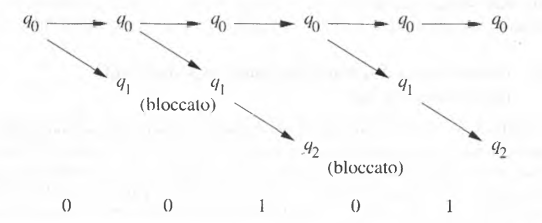
\includegraphics[scale=0.7]{img/nfa.png}
\end{center}
Il funzionamento dell'automa, come si nota nella figura, per la stringa $00101$ è la seguente:
si parte dallo stato inziale $q_0$, quando viene letto 0 si passa a $q_0$ e $q_1$,
poi viene letto il secondo 0 quindi $q_0$ va nuovamente verso $q_0$ e $q_1$ mentre il primo $q_1$ muore non avendo transizioni su 0.\newline
Arriva poi l'1 quindi $q_0$ va solo verso $q_0$ e $q_1$ verso $q_2$ e sarebbe accettante ma l'input non è finito.\newline
Ora arriva 0 e $q_2$ si blocca mentre $q_0$ va sia in $q_0$ che in $q_1$ ed arriva infine un 1 che manda $q_0$ in $q_0$ e $q_1$ in $q_2$
che è accettante e non avendo altri input si è dimostrata l'appartenenza della stringa al linguaggio.
\end{esempio}
Definisco quindi un NFA come una quintupla:
\[ A=(Q,\Sigma,\delta,q_0,F) \]
con, a differenza dei DFA:
\[ \delta:Q\times F\to 2^Q \]
Possiamo ora definire induttivamente $\hat{\delta}$, delta cappuccio che prende in ingresso uno stato e l'intera stringa $w$
e come già visto per i DFA ci sono ben due definizioni:
\begin{itemize}
  \item versione semplificata fornita a lezione in cui si considera una stringa come $w = ax$,
        con $a \in Sigma$ e $x \in Sigma^*$ per cui la definizione di $\hat{delta}$ è:
        \begin{itemize}
          \item \textbf{caso base:} se $w = \epsilon$ si ha $\hat{\delta}(q, \epsilon) = \{q\}$
          \item \textbf{caso passo:} sia $|w| > 0$, $w = ax$ ed avendo $\delta(q, a) = \{p_1, p_2,\dots, p_k\}$
                allora $\hat{\delta}(q, w) = \bigcup _{i = 1} ^ k \hat{\delta}(p_i, x) = \{r_1, r_2,\dots, r_m\}$
        \end{itemize}

  \item versione fornita dal libro in cui si considera $w = xa$, con $x \in Sigma^*$
        e $a \in \Sigma$ per cui la definizione di $\hat{\delta}$ è la seguente:
        \begin{itemize}
          \item \textbf{caso base:} se $|w|=0$ si ha $\hat{\delta}(q,\epsilon) =\{q\}$
          \item \textbf{caso passo:} sia $|w|>0$, $W=xa$, con $a\in\Sigma$ e $x\in\Sigma^*$.\newline
          Posto $\hat{\delta}(q, x)=\{p_1,...,p_k\}$ si ha:
          \[ \hat{\delta}(q, w) = \hat{\delta}(q, xa) = \bigcup _{i = 1} ^ k \delta(p_i, a) \]
        \end{itemize}
\end{itemize}
Il linguaggio accettato dall'automa $NFA$ è il seguente:
\[ L(a) = \{w\in \Sigma^*|\, \hat{\delta}(q_0, q) \cap F \neq \emptyset\} \]
\begin{esempio}
Automa per $L=\{x010y|\,x,y\in\{0,1\}^*\}$ ovvero tutte le stringhe con dentro la sequenza $010$:
\begin{center}
\begin{tikzpicture}[shorten >=1pt,node distance=2cm,on grid,auto]
\node[state, initial] (q_0) {$q_{0}$};
	\node[state] (q_1) [right=of q_0] {$q_{1}$};
	\node[state] (q_2) [right=of q_1] {$q_{2}$};
	\node[state, accepting] (q_3) [right=of q_2] {$q_{3}$};
	\path[->]
	(q_0) edge  node {0} (q_1)
	      edge [loop above] node {0,1} ()
	(q_1) edge  node {1} (q_2)
	(q_2) edge  node {0} (q_3)
	(q_3)     edge [loop above] node {0,1} ();
\end{tikzpicture}
\end{center}
\end{esempio}
Troviamo ora un algoritmo che trasformi un NFA in un DFA.\\
Dall'ultimo esempio ricavo:
\begin{center}
\begin{tabular}{c|c|c}
& 0 & 1\\
\hline
$\emptyset$ & $\emptyset$ & $\emptyset$ \\
\hline
$\to \,\{q_0\}$ & $\{q_0,q_1\}$ & $\{q_0\}$\\
\hline
$\,\{q_1\}$ & $\emptyset$ & $\{q_2\}$\\
\hline
$*\,\{q_2\}$ & $\emptyset$ & $\emptyset$\\
\hline
$\{q_0,q_1\}$ & $\{q_0,q_1\}$ & $\{q_0,q_2\}$\\
\hline
$*\,\{q_0,q_2\}$ & $\{q_0,q_1\}$ & $\{q_0\}$\\
\hline
$*\,\{q_1, q_2\}$ & $\emptyset$ & $\{q_2\}$\\
\hline
$*\,\{q_0,q_1,q_2\}$ & $\{q_0,q_1\}$ & $\{q_0,q_2\}$
\end{tabular}
\end{center}
ovvero:
\begin{center}
\begin{tikzpicture}[shorten >=1pt,node distance=4cm,on grid,auto]
\node[state, initial] (q_0) {$\{q_{0}\}$};
\node[state] (q_1) [right=of q_0] {$\{q_{0}, q_1\}$};
\node[state] (q_2) [right=of q_1] {$\{q_0,q_{2}\}$};
\path[->]
(q_0) edge  node {0} (q_1)
      edge [loop above] node {1} ()
(q_1) edge  node {1} (q_2)
      edge [loop above] node {0} ()
(q_2) edge [bend left =25]  node {0} (q_1)
      edge [bend left =45] node  {1} (q_0);
\end{tikzpicture}
\end{center}
che è il DFA che si era anche prima ottenuto. Si hanno però dei sottoinsiemi mai raggiungibili. Si ha quindi:
\begin{center}
\begin{tabular}{c|c|c}
& 0 & 1\\
\hline
$\to\,\{q_0\}$ & $\{q_0,q_1\}$ & $\{q_0\}$ \\
\hline
$\{q_0,q_1\}$ & $\{q_0,q_1\}$ & $\{q_0,q_2\}$\\
\hline
$\,\{q_0, q_2\}$ & $\{q_0,q_1\}$ & $\{q_0\}$
\end{tabular}
\end{center}
e definendo $\{q_0\}=a, \, \{q_0,q_1\}=b\,\,\, e\,\,\, \{q_0,q_2\}=c$ si avrà:
\begin{center}
\begin{tikzpicture}[shorten >=1pt,node distance=2cm,on grid,auto]
\node[state, initial] (q_0) {$a$};
\node[state] (q_1) [right=of q_0] {$b$};
\node[state, accepting] (q_2) [right=of q_1] {$c$};
\path[->]
(q_0) edge  node {0} (q_1)
      edge [loop above] node {1} ()
(q_1) edge  node {1} (q_2)
      edge [loop above] node {0} ()
(q_2) edge  [bend left =25] node {0} (q_1)
      edge [bend left = 50] node {1} (q_0);
\end{tikzpicture}
\end{center}
Definiamo questo algoritmo che avrà:
\begin{itemize}
\item come input un NFA $N=(Q_n,\Sigma,\delta_N,q_0,F_N)$
\item come output un DFA $D=(Q_D,\Sigma,\delta_D,\{q_0\},F_D)$ tale che $L(D)=L(N)$
\end{itemize}
con:
\begin{itemize}
\item $Q_D=2^{Q_N}$ (quindi se $Q_N=n$ si ha $|Q_D|=2^n$)
\item $F_D=\{S\subseteq Q_n|\, S\cap F_N\neq \emptyset\}$
\item $\forall S\subseteq Q_N$ e $ \forall a \in\Sigma$:
$$\delta_D(S,a)=\cup \delta_n(p,a)$$
per esempio:
$$\delta_D(\{q_0,q_1,q_2\},0)=\delta_N(q_0,0)\cup \delta_N(q_1,0) \cup\delta_N(q_2,0) $$
\end{itemize}

\section{Automi $\epsilon-NFA$}
Si definisce l'$\epsilon-NFA$ come l'automa a stati finiti non deterministici con $\epsilon$ transizioni,
ossia la transizione che permette di saltare i nodi in cui si avanza nel grafo senza consumare caratteri.\newline
Ovviamente questo automa non amplia la classe dei linguaggi accettati dall'automa, ma offre
una certa comodità notazionale e come vedremo gli $\epsilon-NFA$ sono strettamente collegati alle espressioni regolari.

Formalmente denotiamo un $\epsilon-NFA$ con $A = (Q, \Sigma, \delta, q_0, F)$, con gli
stessi argomenti uguali a quelli per il $NFA$ con la differenza che la funzione $\delta$
è definita come $\delta:Q \times \Sigma \cup \{\epsilon\} \to P \subseteq Q$.

Per stabilire le stringhe e i linguaggi accettati da tali automi, dobbiamo introdurre
la funzione $ECLOSE(q)$, per stabilire la chiusura di uno stato rispetto a $\epsilon$, definita induttivamente come:
\begin{itemize}
  \item \textbf{caso base:} lo stato $q$ appartiene a $ECLOSE(q)$
  \item \textbf{caso passo:} se lo stato $p \in ECLOSE(q)$ ed esiste una transizione $\epsilon$ da $p$ a $r$, allora $r \in ECLOSE(q)$.\newline
        Più precisamente, sia $\delta$ la funzione di transizione di un $\epsilon-NFA$: se $p \in ECLOSE(q)$,
        allora $ECLOSE(q)$ contiene anche tutti gli stati in $\delta(p, \epsilon)$.
\end{itemize}
Tramite questa definizione di $ECLOSE$ possiamo definire ora la funzione $\hat{\delta}$ in maniera induttiva:
\begin{itemize}
\item Fare definizione
\end{itemize}

\begin{esempio}
Si ha $ER=a^*b^*c^*$, che genera $L=\{a^nb^mc^k|\,n,m,k\geq 0\}$, l'automa per denotare il linguaggio è il seguente:
\begin{figure}
\caption{Automa $\epsilon-NFA$ per generare il linguaggio $a^nb^mc^k$}
\begin{tikzpicture}[shorten >=1pt,node distance=2cm,on grid,auto]
\node[state, initial] (q_0) {$q_0$};
\node[state] (q_1) [right=of q_0] {$q_1$};
\node[state, accepting] (q_2) [right=of q_1] {$q_2$};
\path[->]
(q_0) edge  node {$\epsilon$} (q_1)
      edge [loop above] node {a} ()
(q_1) edge  node {$\epsilon$} (q_2)
      edge [loop above] node {b} ()
(q_2) edge  [loop above] node {c} ();
\end{tikzpicture}
\end{figure}
Si ha poi le seguenti $ECLOSE$:
\[ E\,CLOSE(q_0)=\{q_0,q_1,q_2\} \]
\[ E\,CLOSE(q_1)=\{q_1,q_2\} \]
\[ E\,CLOSE(q_2)=\{q_2\} \]
Mettendo in tabella l'automa $\epsilon-NFA$ si ha:
\begin{table}
\centering
\caption{Tabella di transizione dell'$epsilon-NFA$}
\begin{tabular}{c|c|c|c}
\toprule & a & b & c\\
\midrule
$*\to\,\{q_0,q_1,q_2\}$ & $\{q_0,q_1,q_2\} = A$ & $\{q_1,q_2\} = B$ & $\{q_2\} = C$\\
$*\{q_1,q_2\}$ & $\emptyset = D$ & $\{q_1,q_2\}$ & $\{q_2\}$\\
$*\{q_2\}$ & $\emptyset$ & $\emptyset$ & $\{q_2\}$\\
$\emptyset$ & $\emptyset$ & $\emptyset$ & $\emptyset$
\end{tabular}
\end{table}
Una rappresentazione formale di come si ottengono le seguenti transizioni nella tabella è la seguente:
\[ \delta_D(\{q_0,q_1,q_2\},a)=E\,CLOSE(\delta_N(q_0,a)\cup \delta_N(q_1,a)\cup \delta_N(q_2,a)) \]
\[ =E\,CLOSE(\{q_0\} \cup \emptyset\cup \emptyset)=E\,CLOSE(\{q_0\}) \]
\[ =E\,CLOSE	(q_0)=\{q_0,q_1,q_2\} \]

\[ \delta_D(\{q_0,q_1,q_2\},B)=E\,CLOSE(\delta_N(q_0,b)\cup \delta_N(q_1,b)\cup \delta_N(q_2,b)) \]
\[ =E\,CLOSE(\emptyset \cup \{q_1\}\cup \emptyset)=E\,CLOSE(\{q_1\}) \]
\[ =E\,CLOSE	(q_1)=\{q_1,q_2\} \]

\[ \delta_D(\{q_0,q_1,q_2\},c)=E\,CLOSE(\delta_N(q_0,c)\cup \delta_N(q_1,c)\cup \delta_N(q_2,c)) \]
\[ =E\,CLOSE(\emptyset \cup \emptyset\cup \{q_2\})=E\,CLOSE(\{q_1\}) \]
\[ =E\,CLOSE	(q_2)=\{q_2\} \]

Si ottiene quindi il seguente NFA:
\begin{figure}
\caption{NFA corrispondente all'$\epsilon-NFA$}
\begin{tikzpicture}[shorten >=1pt,node distance=3cm,on grid,auto]
\node[state, initial, accepting] (q_0) {$A$};
\node[state, accepting] (q_1) [right=of q_0] {$B$};
\node[state, accepting] (q_2) [below=of q_0] {$C$};
\node[state] (q_3) [right=of q_2] {$D$};
\path[->]
(q_0) edge  node {b} (q_1)
      edge  node {c} (q_2)
      edge [loop above] node {a} ()
(q_1) edge  node {c} (q_2)
      edge  node {a} (q_3)
      edge [loop above] node {b} ()
(q_2) edge  node {a,b} (q_3)
      edge [loop below] node {c} ()
(q_3) edge [loop below] node {a,b,c} ();
\end{tikzpicture}
\end{figure}
che diventa il seguente DFA:
\begin{figure}
\caption{Automa DFA corrispondente all'$\epsilon-NFA$}
\begin{tikzpicture}[shorten >=1pt,node distance=3cm,on grid,auto]
\node[state, initial, accepting] (q_0) {$\{q_0,q_1,q_2\}$};
\node[state, accepting] (q_1) [right=of q_0] {$\{q_1,q_2\}$};
\node[state, accepting] (q_2) [below=of q_0] {$\{q_2\}$};
\node[state] (q_3) [right=of q_2] {$q_E$};
\path[->]
(q_0) edge  node {b} (q_1)
      edge  node {c} (q_2)
      edge [loop above] node {a} ()
(q_1) edge  node {c} (q_2)
      edge  node {a} (q_3)
      edge [loop above] node {b} ()
(q_2) edge  node {a,b} (q_3)
      edge [loop below] node {c} ();
\end{tikzpicture}
\end{figure}
\end{esempio}
\end{document}
